\documentclass[10pt,compress,t,notes=noshow, xcolor=table]{beamer}

\input{../../style/preamble}
% Defines macros and environments
 
\title{Interpretable Machine Learning}
% \author{LMU}
%\institute{\href{https://compstat-lmu.github.io/lecture_iml/}{compstat-lmu.github.io/lecture\_iml}}

\def\firstrowcolor{}
\def\secondrowcolor{}
\def\thirdrowcolor{}
\def\fourthrowcolor{}

\definecolor{winter}{RGB} {243,117,108}
\definecolor{spring}{RGB} {121,174,65}
\definecolor{summer}{RGB} {25,188,195}
\definecolor{fall}{RGB} {166,128,185}
\setlength{\leftmargini}{1.5em}
\setlength{\leftmarginii}{1em}
\begin{document}

\titlemeta{
Interpretable Models 1
}{
Extensions of Linear Regression Models
}{
figure/l1_hat
}{
\item Inclusion of high-order and interaction effects
\item Regularization via LASSO
%\item Examples of popular interpretable models
%\item Properties of some interpretable models
%\item Focus on how to interpret them, not on math details
}


\begin{framev}[align=top]{Interaction and High-order Effects}
$$\text{LM Equation: } y = \theta_0 + \theta_1 x_1 + \theta_2 x_2 + \dots + \theta_p x_p + \epsilon$$
Equation above can be extended (polynomial regression) by including
\splitVTT[0.7]{
\spacer[0.6]
\begin{itemizeM}
\item \textbf{high-order effects} which have their own weights\\
$\leadsto$ e.g., quadratic effect: $\theta_{x_j^2} \cdot x_j^2$
\item \textbf{interaction effects} as the product of multiple feat.\\
$\leadsto$ e.g., 2-way interaction: $\theta_{x_i, x_j} \cdot x_i \cdot x_j$
\end{itemizeM}
}{
\spacer[0]
\centering
\begin{scriptsize}
\textbf{Bike Data}\\
\begin{tabular}{lrr}
\hline
Method & $R^2$ & adj. $R^2$ \\
\hline
Simple LM & 0.85 & 0.84 \\
High-order & 0.87 & 0.87 \\
Interaction & 0.96 & 0.93 \\
%    Both Types & 0.96 & 0.93 \\
\hline
\end{tabular}
\end{scriptsize}
\spacer[0]
% code for tables in rsrc/tab_lm_comparison.R
}
\pause\\
\spacer[0.25]
Implications of including high-order and interaction effects:
\begin{itemizeM}
\item Both make the model more flexible but also less interpretable\\
$\leadsto$ More weights to interpret
\item Both need to be specified manually (inconvenient, sometimes infeasible)\\
$\leadsto$ Other ML models often learn them automatically
\item Marginal effect of a feat. cannot be interpreted by single weights anymore\\
$\leadsto$ Feature $x_j$ occurs multiple times (with different weights) in equation
\end{itemizeM}
\end{framev}

\begin{framev}[align=top]{Example: Interaction Effect}
\textbf{Ex.}: Interaction between \code{temp} and \code{season} will affect marginal effect of \code{temp}% with (right) and without (left) interaction.
\spacer[0.25]
\splitVTT[0.65]{
\spacer[0]
\image{figure/lm_main_vs_interaction_effects.pdf}
\spacer[0]
}{
\spacer[0]
\centering
\begin{scriptsize}
%\begin{table}[ht]
\only<2->{\def\firstrowcolor{\rowcolor{lightgray}}}
\only<3>{\def\secondrowcolor{\rowcolor{lightgray}}}
\only<4>{\def\thirdrowcolor{\rowcolor{lightgray}}}
\only<5>{\def\fourthrowcolor{\rowcolor{lightgray}}}
\begin{tabular}{rr}
\hline
& Weights \\
\hline
(Intercept) & 3453.9 \\ 
seasonSPRING & 1317.0 \\ 
seasonSUMMER & 4894.1 \\ 
seasonFALL & -114.2 \\ 
\firstrowcolor temp & 160.5 \\ 
hum & -37.6 \\ 
windspeed & -61.9 \\ 
days\_since\_2011 & 4.9 \\
\hline
\secondrowcolor seasonSPRING:temp & -50.7 \\ 
\thirdrowcolor seasonSUMMER:temp & -222.0 \\ 
\fourthrowcolor seasonFALL:temp & 27.2 \\ 
\hline
\end{tabular}
%\end{table}
\end{scriptsize}
\spacer[0]
}
\pause
\spacer[0.25]
\splitVTT[0.65]{
\textbf{Interpretation}: If \code{temp} increases by 1 $^{\circ}$C, \\ bike rentals
\begin{itemize}[<+->]
\item increase by 160.5 in \code{WINTER} (reference)
\item increase by 109.8 (= 160.5 - 50.7) in \code{SPRING}
\item decrease by -61.5 (= 160.5 - 222) in \code{SUMMER}
\item increase by 187.7 (= 160.5 + 27.2) in \code{FALL}
\end{itemize} %\\\vspace*{0.2cm}
}{
% \lz
% \only<6>{\textbf{Note:}
% Temperature values (on x-axis) depend on \code{season}\\
% $\leadsto$ not acknowledged by LM\\
% $\leadsto$ misleading interpretation due to extrapolation in regions with few points (e.g. low \code{temp} in \code{SUMMER})
% }
}
%Value ranges of temperature differ depending on the season $\leadsto$ not acknowledged by LM
\end{framev}


\begin{framev}[align=top,fs=small]{Example: Quadratic Effect}
\textbf{Ex.}: Adding quadratic effect for \code{temp} \only<2>{(left) and interaction with \code{season} (right)}
\spacer[0.25]
\splitVTT[0.7]{
\spacer[0]

\includegraphics[width=0.5\textwidth, trim=0cm 0.1cm 10.4cm 0cm, clip]{figure/poly_main_vs_interaction_effects.pdf}\invisible<1>{
\includegraphics[width=0.5\textwidth, trim=10cm 0.1cm 0.4cm 0cm, clip]{figure/poly_main_vs_interaction_effects.pdf}}
%
\includegraphics[width = \textwidth]{figure/poly_main_vs_interaction_effects.pdf}
%\begin{columns}[totalwidth=\textwidth]
%\begin{center}
%\adjincludegraphics[width=\textwidth, trim={0 0 {.55\width} 0}, clip]{figure/poly_main_vs_interaction_effects.pdf}
\\
\textbf{Interpretation}: Not linear anymore!
\begin{itemizeS}
\only<1>{\item \code{temp} depends on two weights: $280.2 \cdot x_{temp} - 5.6 \cdot x_{temp}^2$}
\item<2> \code{temp} depends on multiple weights due to \code{season}:\\
$\leadsto$ \code{WINTER}: \\${\color{winter}39.1} \cdot x_{temp} + {\color{winter}8.6} \cdot x_{temp}^2$ \\
$\leadsto$ \code{SPRING}:\\
$({\color{winter}39.1} {\color{spring}+407.4}) \cdot x_{temp} + ({\color{winter}8.6} {\color{spring} - 18.7}) \cdot x_{temp}^2$ \\
$\leadsto$ \code{SUMMER}:\\ $({\color{winter}39.1} {\color{summer}+801.1}) \cdot x_{temp} + ({\color{winter}8.6} {\color{summer} - 27.2}) \cdot x_{temp}^2$ \\
$\leadsto$ \code{FALL}: \\$({\color{winter}39.1} {\color{fall}+217.4}) \cdot x_{temp} + ({\color{winter}8.6} {\color{fall} - 11.3}) \cdot x_{temp}^2$
\end{itemizeS}
}{
\spacer[0]
%\hfill
\begin{scriptsize}
% \begin{table}[ht]
% %\centering

\def\firstrowcolor{\rowcolor{lightgray}}%
\def\secondrowcolor{\rowcolor{spring}}%
\def\thirdrowcolor{\rowcolor{summer}}%
\def\fourthrowcolor{\rowcolor{fall}}%

\only<1>{%
%\addtolength{\tabcolsep}{-1pt}
\begin{tabular}{rr}
\hline
& Weights \\
\hline
(Intercept) & 3094.1 \\ 
seasonSPRING & 619.2 \\ 
seasonSUMMER & 284.6 \\ 
seasonFALL & 123.1 \\ 
hum & -36.4 \\ 
windspeed & -65.7 \\ 
days\_since\_2011 & 4.7 \\ 
\firstrowcolor temp & 280.2 \\ 
\firstrowcolor temp$^2$ & -5.6 \\ 
\hline
\end{tabular}%
%\addtolength{\tabcolsep}{1pt}
}
% \end{table}
\only<2>{%
\def\firstrowcolor{\rowcolor{winter}}%
\addtolength{\tabcolsep}{-3pt}%
\begin{tabular}{rr}
\hline
& Weights \\
\hline
(Intercept) & 3802.1 \\ 
seasonSPRING & -1345.1 \\ 
seasonSUMMER & -6006.3 \\ 
seasonFALL & -681.4 \\ 
hum & -38.9 \\ 
windspeed & -64.1 \\ 
days\_since\_2011 & 4.8 \\ 
\firstrowcolor temp & 39.1 \\ 
\firstrowcolor temp$^2$ & 8.6 \\ 
\hline
\hline
\secondrowcolor seasonSPRING:temp & 407.4 \\ 
\secondrowcolor seasonSPRING:temp$^2$ & -18.7 \\ 
\thirdrowcolor seasonSUMMER:temp & 801.1 \\ 
\thirdrowcolor seasonSUMMER:temp$^2$ & -27.2 \\ 
\fourthrowcolor seasonFALL:temp & 217.4 \\ 
\fourthrowcolor seasonFALL:temp$^2$ & -11.3 \\ 
\hline
\end{tabular}%
\addtolength{\tabcolsep}{3pt}
}%
%Table: Weights for main effect model
\end{scriptsize}
%\end{center}
}
\end{framev}


\begin{framev}[align=top]{Regularization via LASSO \furtherreading{TIBSHIRANI1996}}
\splitVTT[0.6]{
\spacer[0.6]
\begin{itemizeM}
\item LASSO adds an $L_1$-norm penalization term ($\lambda||\theta||_1$) to least squares optimization problem
\begin{itemizeS}
\item[$\leadsto$] Shrinks some feature weights to zero\\
(feature selection)
\item[$\leadsto$] Sparser models (fewer features): \\
more interpretable
\end{itemizeS}
%Aim: Feature selection (sparsity) and regularization of feature weights
\item Penalization parameter $\lambda$ must be chosen (e.g., by CV) %or depending on the number of features to keep
\end{itemizeM}
\spacer[0.25]
$$
min_{\theta} \bigg(\underbrace{\frac{1}{n} \sum_{i=1}^{n} (y^{(i)} - {\xi}^{\top} \theta)^2}_\text{Least square estimate for LM} + \lambda||\theta||_1\bigg) 
$$
}{
\spacer[0]
\imageC[0.8]{figure/l1_hat.png}
\imageC[0.8]{figure/lm_example}
}
\end{framev}


\begin{framev}[align=top]{Regularization via LASSO \furtherreading{TIBSHIRANI1996}}
\textbf{Example} (interpretation of weights analogous to LM):
\begin{itemizeM}
\item LASSO with main effects and interaction \code{temp} with \code{season}
\end{itemizeM}
\splitVTT[0.65]{
\spacer[0.6]
\begin{itemizeM}
\item $\lambda$ is chosen $\leadsto$ 6 selected features ($\neq 0$)
\item LASSO shrinks weights of single categories separately (due to dummy encoding)\\
$\leadsto$ No feature selection of whole categorical features (only w.r.t. category levels)\\
$\leadsto$ Solution: group LASSO \furtherreading{YUANLIN2006}
\end{itemizeM}
\spacer[0.25]
\imageC[0.6]{figure/reg_lm_plot_interpreted.pdf}
}{
\spacer[0]
\begin{scriptsize}
\centering
\begin{tabular}{rr}
\hline
& Weights \\
\hline
(Intercept) & 3135.2 \\ 
seasonSPRING & 767.4 \\ 
seasonSUMMER & 0.0 \\ 
seasonFALL & 0.0 \\ 
temp & 116.7 \\ 
hum & -28.9 \\ 
windspeed & -50.5 \\ 
days\_since\_2011 & 4.8 \\ 
\hline
seasonSPRING:temp & 0.0 \\ 
seasonSUMMER:temp & 0.0 \\ 
seasonFALL:temp & 30.2 \\ 
\hline
\end{tabular}
%\end{table}
% \begin{table}[ht]
% \centering
% \begin{tabular}{rr}
%   \hline
%  & Weights \\ 
%   \hline
% (Intercept) & 2665.50 \\ 
%   seasonSPRING & 489.34 \\ 
%   seasonSUMMER & 0.00 \\ 
%   seasonFALL & 0.00 \\ 
%   hum & -19.44 \\ 
%   windspeed & -35.54 \\ 
%   days\_since\_2011 & 4.71 \\ 
%   poly(temp, 2)1 & 109.25 \\ 
%   poly(temp, 2)2 & 0.00 \\ 
%   \hline
% \end{tabular}
% \end{table}
\end{scriptsize}
}
%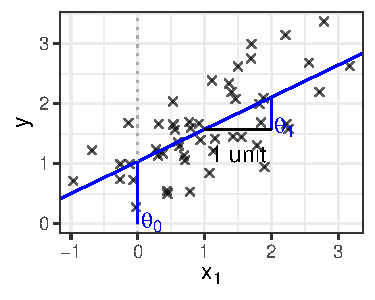
\includegraphics[width = 0.8\textwidth]{figure/reg_lm_plot_interpreted.pdf}
\end{framev}
\endlecture

\end{document}
